

\tikzset{every picture/.style={line width=0.75pt}} %set default line width to 0.75pt        

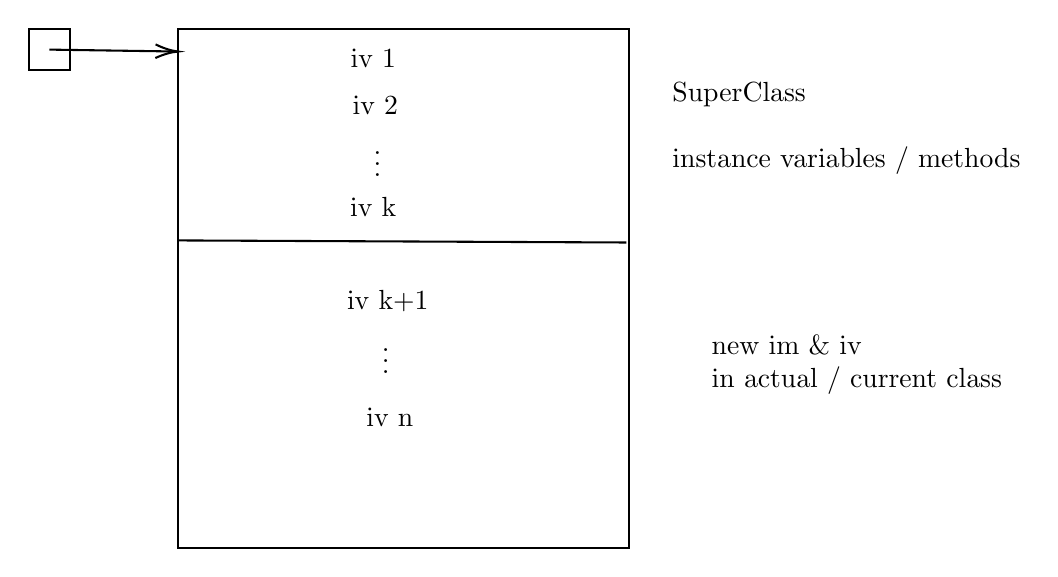
\begin{tikzpicture}[x=0.75pt,y=0.75pt,yscale=-1,xscale=1]
%uncomment if require: \path (0,300); %set diagram left start at 0, and has height of 300

%Shape: Rectangle [id:dp6411994266752609] 
\draw   (182,27.93) -- (399,27.93) -- (399,277.93) -- (182,277.93) -- cycle ;
%Shape: Square [id:dp3458024066933377] 
\draw   (110,28) -- (130,28) -- (130,48) -- (110,48) -- cycle ;
%Straight Lines [id:da4649876373916405] 
\draw    (120,38) -- (180,38.9) ;
\draw [shift={(182,38.93)}, rotate = 180.86] [color={rgb, 255:red, 0; green, 0; blue, 0 }  ][line width=0.75]    (10.93,-3.29) .. controls (6.95,-1.4) and (3.31,-0.3) .. (0,0) .. controls (3.31,0.3) and (6.95,1.4) .. (10.93,3.29)   ;

%Straight Lines [id:da2372718857026357] 
\draw    (182,129.93) -- (398,130.93) ;



% Text Node
\draw (276,42) node  [align=left] {iv 1};
% Text Node
\draw (504,76) node  [align=left] {SuperClass\\\\instance variables / methods};
% Text Node
\draw (509,190) node  [align=left] {new im \& iv\\in actual / current class};
% Text Node
\draw (277,65) node  [align=left] {iv 2};
% Text Node
\draw (276,114) node  [align=left] {iv k};
% Text Node
\draw (278,89) node   {$\vdots $};
% Text Node
\draw (283,159) node  [align=left] {iv k+1};
% Text Node
\draw (284,215) node  [align=left] {iv n};
% Text Node
\draw (282,184) node   {$\vdots $};


\end{tikzpicture}
